
\subsubsection{01.10.14}

\begin{enumerate}
	\item The time of beginning and ending of the congregation:
	18:00 - 21:30
	\item Purposes of the congregation:
	\begin{enumerate}
		\item To chose and create wheelbase of our robot.
		
		\item Write a simple program to control motions of the robot by means of joystick.
		
	\end{enumerate}
	
	\item Results:
	\begin{enumerate}
		\item Weelbase was created:
		\begin{enumerate}
			\item Preference was given to the omni- wheels with a roller disposed at an angle of 45 degrees to the direction of rotation. However, we didn't have such weels. This is why we used usual weels instead of omni-weels.
			
			\item We tried to put the heaviest parts as close to the earth, as possible. So, the battery, NXT microcontroller and the drivers of the motors and servo-motors were located in the lower part of the robot. 
			
			\item Wires could accidentally climb out and cling to the other robots or to the moving parts of the robot itself. So we decided protect the wires from the bottom.
			
			\begin{figure}[H]
				\begin{minipage}[h]{0.2\linewidth}
					\center  
				\end{minipage}
				\begin{minipage}[h]{0.6\linewidth}
					\center{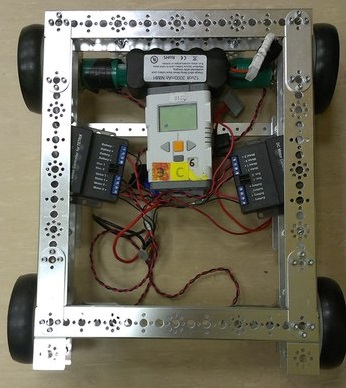
\includegraphics[scale=0.5]{days/01.10.14/images/01}}
					\caption{The ideas for fixing the movable basket: 1)A capture, that look likes as russian letter "П" 2)Capture with hooks}
				\end{minipage}
			\end{figure}
			
		\end{enumerate}
		
		\item There was idea to create lift like a conveyer belt. Such system could lead to the capture of balls fixed on the body of the robot, and raise only balls. So, there were some ideas:
		\begin{enumerate}
			\item Conveyer belt with baskets, that are located at equal distances
			\item Sliding hollow cylinder in which axes that lift balls can move.			
			\begin{figure}[H]
				\begin{minipage}[h]{0.2\linewidth}
					\center  
				\end{minipage}
				\begin{minipage}[h]{0.6\linewidth}
					\center{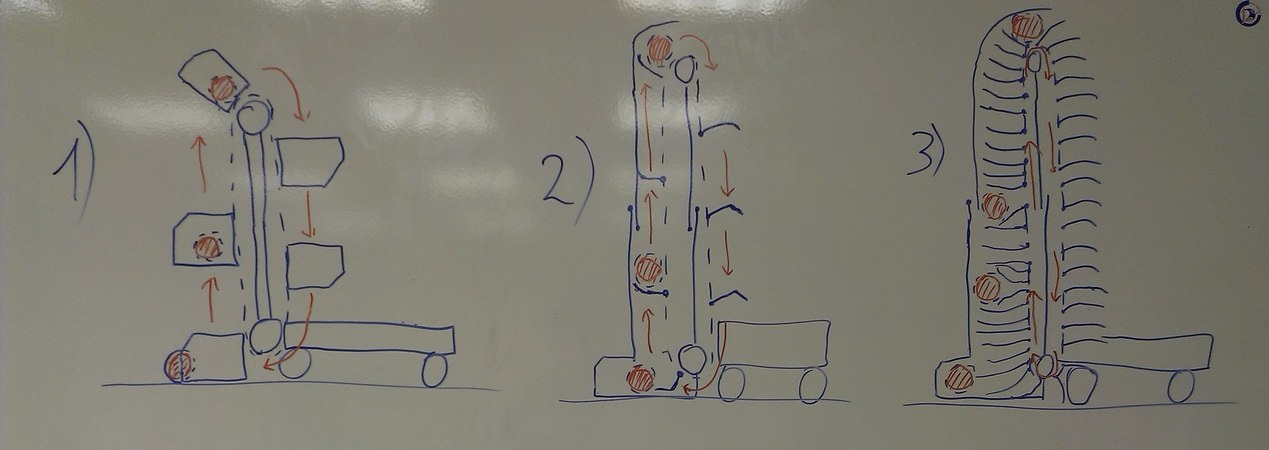
\includegraphics[scale=0.25]{days/01.10.14/images/02}}
					\caption{Ideas for ball's lift: 1)Conveyer with baskets 2)Construction with sliding hollow cylinder
				\end{minipage}
			\end{figure}
			
		\end{enumerate}
		
	\end{enumerate}
	
	\item Results: 
	\begin{enumerate}
		\item Wheelbase of the robot was assembled.
		
		\item Program wasn't realised.
		
	\end{enumerate}
	
	\item Tasks for the next congregations:
	\begin{enumerate}
		\item Realise robot's programm.
		
		\item Install underbody protection.
		
	\end{enumerate}     
\end{enumerate}
\fillpage

